\documentclass[a4paper, 12pt]{article}

% Essential packages
\usepackage[T1, T2A]{fontenc}
\usepackage[utf8]{inputenc}
\usepackage[russian, english]{babel}
\usepackage{graphicx}
\usepackage{geometry}
\usepackage{amsmath}
\usepackage{amsfonts}
\usepackage{amssymb}
\usepackage{hyperref}
\usepackage{indentfirst}
\usepackage{authblk}
\usepackage{gensymb}
\usepackage{listings}
\usepackage{xcolor}
\usepackage{minted}
\usepackage{float}
\usepackage{caption}
\usepackage[russian]{babel}

\captionsetup[figure]{name=Рис., aboveskip=0.5pt, belowskip=0.5pt}


\captionsetup[table]{name=Табл., aboveskip=1pt, belowskip=0.5pt}

\setminted{
    breaklines=true,
    breakautoindent=true,
    breakindent=20pt,
    fontsize=\small,  % опционально: уменьшает шрифт
    frame=lines,      % опционально: рамка для наглядности
    framesep=2mm
}

% \lstset{
%     language=Matlab,
%     basicstyle=\ttfamily\small,
%     numbers=left,
%     numberstyle=\tiny,
%     stepnumber=1,
%     breaklines=true,
%     keywordstyle=\color{blue},
%     commentstyle=\color{green!50!black},
%     stringstyle=\color{red},
%     frame=single
% }

% Page margins setup
\geometry{left=2cm, right=2cm, bottom=2cm, top=2cm}

% Hyperlink setup
\hypersetup{
    colorlinks=true,
    linkcolor=blue,
    filecolor=magenta,
    urlcolor=cyan
}

\begin{document}
\begin{titlepage}

\begin{minipage}[c]{0.65\textwidth}
    {\vspace{0.5cm}\Large\textbf{УНИВЕРСИТЕТ ИТМО}}\\
    \small{Факультет Систем Управления и Робототехники}
\end{minipage}
\begin{minipage}[c]{0.35\textwidth}
    \begin{flushright}
        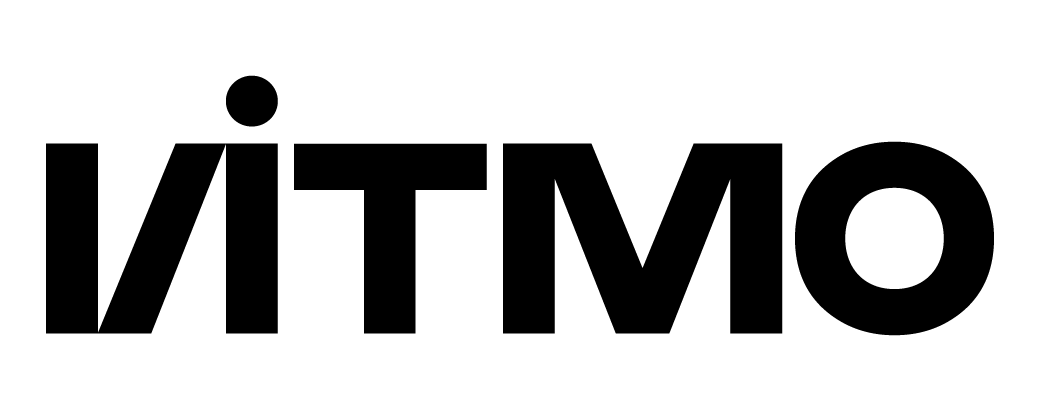
\includegraphics[width=0.8\textwidth]{itmo.png}
    \end{flushright}
\end{minipage}

\vfill
\vfill

\begin{center}
\textbf{\Large Лабораторная работа №2 <<Непрерывное преобразование Фурье>>}\\[5pt]
{\large Частотные методы}


\vfill
\vfill

\begin{flushleft}
    Выполнили:\\
    \text{Бурдасова Виктория: 465306}\\
    \text{Жаворонков Пётр: 465877}\\
    \text{Беляев Александр: 465203}
\end{flushleft}

\vfill

Санкт-Петербург\\
2026

\end{center}
\end{titlepage}
\renewcommand*\contentsname{Содержание}
\tableofcontents

\newpage

\section{Вещественные функции}

В этом задании надо рассмотреть следующие функции $f:\mathbb{R} \to \mathbb{R}$:

\begin{enumerate}
    \item Прямоугольная функция:
    \[
    f(t)=
    \begin{cases}
    a, & |t|\leq b,\\
    0, & |t|>b.
    \end{cases}
    \]

    \item Треугольная функция:
    \[
    f(t)=
    \begin{cases}
    a - \left| \dfrac{a t}{b} \right|, & |t|\leq b,\\
    0, & |t|>b.
    \end{cases}
    \]

    \item Кардинальный синус:
    \[
    f(t)=a\,\mathrm{sinc}(bt).
    \]

    \item Функция Гаусса:
    \[
    f(t)=a e^{-b t^2}.
    \]

    \item Двустороннее затухание:
    \[
    f(t)=a e^{-b|t|}.
    \]
\end{enumerate}

Также для каждой из функций $f(t)$ необходимо провести исследование её Фурье-образа $\hat{f}(\nu)$ и свойств преобразования Фурье. Для этого:

\begin{enumerate}
    \item Нужно привести аналитические выражения оригинала функции $f(t)$ и её Фурье-образа $\hat{f}(\nu)$ в общем виде (без выбора конкретных значений $a$ и $b$).
    
    \begin{enumerate}
        \item Для функций 1, 2 и 5 необходимо привести вывод соответствующих аналитических выражений с выкладками.
        \item Для функций 3 и 4 достаточно привести результат. Для функции 3 рекомендуется воспользоваться свойствами преобразования Фурье, функцию 4 же допустимо взять из готовых таблиц преобразований Фурье в специализированной литературе.
    \end{enumerate}

    \item Задаться не менее чем тремя наборами значений параметров $a, b > 0$ и построить графики оригинала функции $f(t)$ и графики Фурье-образа $\hat{f}(\nu)$ для выбранных значений.
    
    \item Проанализировать полученные результаты с точки зрения свойств преобразования Фурье: определить для каждого из параметров $a$ и $b$, каким свойством преобразования Фурье обоснованы изменения в функции-оригинале и её образе, связанные с вариацией данного параметра.

    \item Проверить выполнение равенства Парсеваля.
\end{enumerate}

\subsection{Прямоугольная функция}

Данная функция задаётся формулой:
\[
    \Pi(t)=
    \begin{cases}
    a, & |t|\leq b,\\
    0, & |t|>b.
    \end{cases}
\]

Фурье-образ функции вычисляется по общей формуле:
\[
\hat{f}(\nu) = \int^{\infty}_{-\infty} f(t)e^{-2\pi i \nu t}dt
\]

Вычислим Фурье-образ прямоугольной функции:
\[
\hat{\Pi}(\nu) = \int^{\infty}_{-\infty} \Pi(t)e^{-2\pi i \nu t}dt
\]

Но $\Pi(t) = 0,\ t\in (-\infty; -b)\cup (b; \infty)$. Значит, 
\[
\hat{\Pi}(\nu) = \int^b_{-b} \Pi(t)e^{-2\pi i \nu t}dt =  \int^b_{-b} a \cdot e^{-2\pi i \nu t}dt = a \cdot \int^b_{-b}e^{-2\pi i \nu t}dt = -a \cdot \frac{e^{-2\pi i \nu t}}{2\pi i \nu} \Bigg|^{b}_{-b}
\]
Продолжая вычисления, получим:
\[
\hat{\Pi}(\nu) = a \cdot \frac{e^{2\pi i \nu b} - e^{-2\pi i \nu b}}{2\pi i \nu} = 2b \cdot a \cdot \frac{e^{2\pi i \nu b} - e^{-2\pi i \nu b}}{2b\cdot2\pi i \nu} = 2ab \cdot \frac{e^{ i (2\pi \nu b)} - e^{-i(2\pi \nu b)}}{2i\cdot (2\pi  \nu b)} = 2ab \cdot sinc (2\pi \nu b) 
\]
Итого: 

\[
\hat{\Pi}(\nu) = 2ab \cdot sinc (2\nu b) 
\]

Теперь зададимся тремя наборами значений $a, b > 0$ для прямоугольной функции. Пусть $a, b = \{(1; \frac{1}{2}),\ (1; 1),\ (2;1)\}$.\\

Построим графики для оригиналов и Фурье-образов следующих функций: 
\[
    \Pi_1(t)=
    \begin{cases}
    1, & |t|\leq \frac{1}{2},\\
    0, & |t|> \frac{1}{2}.
    \end{cases}\ \ \ \
\hat{\Pi_1}(\nu) = sinc (\nu) 
\]\\[1pt]
\[
    \Pi_2(t)=
    \begin{cases}
    1, & |t|\leq 1,\\
    0, & |t| > 1.
    \end{cases}\ \ \ \
\hat{\Pi_2}(\nu) = 2\cdot sinc (2\nu) 
\]\\[1pt]
\[
    \Pi_3(t)=
    \begin{cases}
    2, & |t|\leq 1,\\
    0, & |t|>1.
    \end{cases}\ \ \ \
\hat{\Pi_3}(\nu) = 4 \cdot sinc (2\nu) 
\]\\

\begin{figure}[H] 
    \includegraphics[width=1\textwidth]{graphs/111.pdf}
    \caption{Графики оригиналов функций}
\end{figure}

\begin{figure}[H] 
    \includegraphics[width=1\textwidth]{graphs/112.pdf}
    \caption{Графики Фурье-образов функций}
\end{figure}

\newpage
Теперь проанализируем полученные результаты. Мы получили следующую формулу в общем виде для прямоугольной функции:
\[
\hat{\Pi}(\nu) = 2ab \cdot sinc (2 \nu b) 
\]

Параметр $a$ в оригинале функции влияет на промежуток $t \in (-b; b)$: функция равна его значению на этом промежутке. Следовательно, с увеличением параметра $a$ увеличивается значение функции на промежутке $t \in (-b; b)$.\\

Параметр $b$ в оригинале функции задаёт промежуток, на котром функция равна параметру $a$. С увеличением $b$ увеличивается промежуток, на котором оригинал функции равен $a$.\\

Параметр $a$ в Фурье-образе увеличивает амплитуду функции в $a$ раз.\\

Параметр $b$ в Фурье-образе увеличивает амплитуду функции в $b$ раз. А также сжимает функцию в $b$ раз.\\

Теперь проверим равенство Парсеваля. Оно вычисляется по формуле:
\[
||f||_2=||\mathcal{F}f||_2
\]

\[
||f|| = \sqrt{\int_{-b}^b a^2dt} = \sqrt{a^2t\Bigg|_{-b}^{b}} = \sqrt{a^2b - a^2(-b)} = \sqrt{2a^2b}
\]

\[
\|\hat{\Pi}\|_2^2 =
\int_{-\infty}^{\infty}
|2ab \, \mathrm{sinc}(2b\nu)|^2 \, d\nu
=
4a^2 b^2
\int_{-\infty}^{\infty}
\mathrm{sinc}^2(2b\nu)\, d\nu = 4a^2 b^2 \cdot \frac{1}{2b}
= 2a^2 b.
\]

\[
\|\hat{\Pi}\|_2 = \sqrt{2a^2b}
\]

Равенство Парсеваля выполняется.

\subsection{Треугольная функция}
Теперь рассмотрим треугольную функцию, в общем виде она задаётся так:

\[
    f(t)=
    \begin{cases}
    a - \left| \dfrac{a t}{b} \right|, & |t|\leq b,\\
    0, & |t|>b.
    \end{cases}
\]

Найдём её Фурье-образ:

\[
\hat{f}(\nu) = \int^{\infty}_{-\infty} f(t)e^{-2\pi i \nu t}dt
\]

Но $f(t) = 0,\ t\in (-\infty; -b)\cup (b; \infty)$. Значит, 

\[
\hat{f}(\nu) = \int^b_{-b}f(t)e^{-2\pi i \nu t}dt = \int^b_{-b} \left(a - \left| \dfrac{a t}{b} \right|\right)e^{-2\pi i \nu t}dt = \int_{-b}^0\left(a + \frac{a t}{b}\right)e^{-2\pi i \nu t}dt + \int_0^b\left(a - \frac{a t}{b}\right)e^{-2\pi i \nu t}dt
\]

\[
\hat{f}(\nu) = \left( -\frac{a}{2\pi i \nu} \right) \left( e^{-2\pi i \nu t} + \frac{te^{-2\pi i \nu t}}{b} + \frac{e^{-2\pi i \nu t}}{b(2\pi i \nu)} \right)\Bigg|_{-b}^0 
+
\left( -\frac{a}{2\pi i \nu} \right) \left( e^{-2\pi i \nu t} - \frac{te^{-2\pi i \nu t}}{b} - \frac{e^{-2\pi i \nu t}}{b(2\pi i \nu)} \right)\Bigg|_{0}^b
\]

% \[
% \hat{f}(\nu) = \left( -\frac{a}{2\pi i \nu}\right) \left( 1 + \frac{1}{b(2\pi i \nu)} - \frac{e^{2\pi i \nu b}}{b(2\pi i \nu)} -\frac{e^{-2\pi i \nu b}}{b(2\pi i \nu)} - 1 + \frac{1}{b(2\pi i \nu)} \right)
% \]

\[
\hat{f}(\nu) 
= 
\left( -\frac{a}{2\pi i \nu}\right) \left(\frac{1}{b(\pi i \nu)} - \frac{e^{2\pi i \nu b} + e^{-2\pi i \nu b}}{b(2\pi i \nu)} \right) 
=
\left( -\frac{a}{2\pi i \nu}\right) \left(\frac{1}{b(\pi i \nu)} - \frac{cos(2\pi \nu b)}{b(\pi i \nu)} \right)
\]

\[
\hat{f}(\nu) =
\left(\frac{a}{2b\pi^2\nu^2} \right) \left( 1 - \cos(2b \pi \nu) \right) = \left(\frac{a}{2b\pi^2\nu^2} \right) \left(2 \sin^2(b\pi\nu)  \right) = ab\cdot \frac{\sin^2(b \pi \nu)}{(b \pi \nu)^2}
\]\\[1pt]

Итого:
\[
\hat{f}(\nu) = ab \cdot sinc^2(b \nu)
\]\\

Теперь зададимся тремя наборами значений $a, b > 0$ для прямоугольной функции. Пусть $a, b = \{(1; 1),\ (2; 1),\ (1;2)\}$.\\

Построим графики оригиналов и их Фурье-образов для функций:

\[
    f_1(t)=
    \begin{cases}
    1 - \left| t \right|, & |t|\leq 1,\\
    0, & |t|>1.
    \end{cases}\ \ \ \
\hat{f_1}(\nu) = sinc^2(\nu)
\]\\[1pt]

\[
    f_2(t)=
    \begin{cases}
    2 - \left|2t\right|, & |t|\leq 1,\\
    0, & |t|>1.
    \end{cases}\ \ \ \
\hat{f_2}(\nu) = 2 \cdot sinc^2(\nu)
\]\\[1pt]

\[
    f_3(t)=
    \begin{cases}
    1 - \left| \dfrac{t}{2} \right|, & |t|\leq 2,\\
    0, & |t|>2.
    \end{cases}\ \ \ \
\hat{f_3}(\nu) = 2 \cdot sinc^2(2\nu)
\]\\[1pt]

\begin{figure}[H] 
    \includegraphics[width=1\textwidth]{graphs/121.pdf}
    \caption{Графики оригиналов функций}
\end{figure}

\begin{figure}[H] 
    \includegraphics[width=1\textwidth]{graphs/122.pdf}
    \caption{Графики Фурье-образов функций}
\end{figure}

Теперь проанализируем полученные результаты. Мы получили следующую формулу в общем виде для треугольной функции:
\[
\hat{f}(\nu) = ab \cdot sinc^2(b \nu)
\]

Параметр $a$ в оригинале функции влияет на растяжение функции вдоль оси $OY$. Чем больше $a$ -- тем <<выше>> треугольник, при этом его ширина сохраняется.\\

Параметр $b$ в оригинале функции растягивает или сжимает её вдоль оси $OX$. С увеличением $b$ <<треугольник растягивается>> вдоль $OX$.\\

Параметр $a$ в Фурье-образе увеличивает амплитуду функции в $a$ раз. А также растягивает её вдоль оси $OY$\\

Параметр $b$ в Фурье-образе увеличивает амплитуду функции в $b$ раз. А также сжимает функцию в $b$ раз вдоль оси $OX$.\\

Проверим выполнение равенства Парсеваля.

\[
f(t)=
\begin{cases}
a-\left|\dfrac{at}{b}\right|, & |t|\le b,\\
0, & |t|>b
\end{cases}
\qquad
\hat f(\nu)=ab\,\mathrm{sinc}^2(b\nu),
\qquad
\mathrm{sinc}(x)=\dfrac{\sin(\pi x)}{\pi x}
\]

Проверим равенство Парсеваля
\[
\int_{-\infty}^{\infty}|f(t)|^2dt
=
\int_{-\infty}^{\infty}|\hat f(\nu)|^2d\nu .
\]

Функция чётная, поэтому
\[
\int_{-\infty}^{\infty}|f(t)|^2dt
=
2\int_0^b a^2\left(1-\frac{t}{b}\right)^2dt =
2a^2\frac{b}{3}
=
\frac{2}{3}a^2b.
\]

\[
\int_{-\infty}^{\infty}|\hat f(\nu)|^2d\nu
=
a^2b^2
\int_{-\infty}^{\infty}\mathrm{sinc}^4(b\nu)d\nu=
a^2b\cdot\frac{2}{3}
=
\frac{2}{3}a^2b.
\]

Получим, что равенство выполняется.

\subsection{Кардинальный синус}
Теперь рассмотрим функцию, которая задаётся так:
\[
    f(t)=a\,\mathrm{sinc}(bt)
\]

Найдём её Фурье-образ:
\begin{equation}
    \hat{f}(\nu) = \int^{\infty}_{-\infty} f(t)e^{-2\pi i \nu t}dt = \int^{\infty}_{-\infty} a\,\mathrm{sinc}(bt) e^{-2\pi i \nu t}dt = \frac{a}{b}\Pi\!\left(\frac{v}{b}\right)
    \label{equation: sinc img}    
\end{equation}



\[
\hat f(v) =
\begin{cases}
\dfrac{a}{b}, & |\nu|\le \dfrac{b}{2}\\[10pt]
0, & |\nu|>\dfrac{b}{2}
\end{cases}
\]\\

Теперь зададимся тремя наборами значений $a, b > 0$ для прямоугольной функции. Пусть $a, b = \{(1; 1),\ (1; 3),\ (3;1)\}$.\\

Построим графики для оригиналов и Фурье-образов следующих функций:

\[
{\Pi_1}(t) = sinc (t) 
    \ \ \ \
    \hat{\Pi_1}(\nu)=
    \begin{cases}
    1, & |\nu|\leq \frac{1}{2},\\[3pt]
    0, & |\nu|> \frac{1}{2}.
    \end{cases}\\[1pt]
\]

\[
{\Pi_2}(t) = sinc (3t) 
    \ \ \ \
    \hat{\Pi_2}(\nu)=
    \begin{cases}
    \frac{1}{3}, & |\nu|\leq \frac{3}{2},\\[3pt]
    0, & |\nu|> \frac{3}{2}.
    \end{cases}\\[1pt]
\]

\[
{\Pi_3}(t) = 3sinc (t) 
    \ \ \ \
    \hat{\Pi_3}(\nu)=
    \begin{cases}
    3, & |\nu|\leq \frac{1}{2},\\[3pt]
    0, & |\nu|> \frac{1}{2}.
    \end{cases}\\[1pt] 
\]\\

\begin{figure}[H] 
    \includegraphics[width=1\textwidth]{graphs/131.pdf}
    \caption{Графики оригиналов функций}
\end{figure}

\begin{figure}[H] 
    \includegraphics[width=1\textwidth]{graphs/132.pdf}
    \caption{Графики Фурье-образов функций}
\end{figure}

Параметр $a$ в оригинале функции увеличивает амплитуду функции в $a$ раз. То есть растягивает её в $a$ раз вдоль оси $OY$\\

Параметр $b$ в оригинале функции сжимает функцию в $b$ раз вдоль оси $OX$.\\

Параметр $a$ в образе влияет на промежуток $t \in (\frac{-b}{2}; \frac{b}{2})$: функция равна $\frac{a}{b}$ на этом промежутке. Следовательно, с увеличением параметра $a$ увеличивается значение функции на промежутке $t \in (\frac{-b}{2}; \frac{b}{2})$.\\

Параметр $b$ в образе функции задаёт промежуток, на котором функция равна параметру $\frac{a}{b}$. С увеличением $b$ увеличивается промежуток, на котором оригинал функции равен $\frac{a}{b}$.\\

Выполним проверку равенства Парсеваля:

\[
\int_{-\infty}^{\infty}|f(t)|^2dt
=
a^2\int_{-\infty}^{\infty}sinc^2(bt)\,dt =\frac{a^2}{b}.
\]

\[
\int_{-\infty}^{\infty}|\hat f(\nu)|^2d\nu
=
\int_{-b/2}^{b/2}\frac{a^2}{b^2}\,d\nu =
\frac{a^2}{b}
\]

Получим, что равенство Парсеваля выполняется.

\subsection{Функция Гаусса}
Теперь рассмотрим функцию, которая задаётся так:
\[
    f(t) = ae^{-bt^2}
\]

Фурье-образ функции Гаусса:
\[
\hat{f}(\omega) = \frac{a}{\sqrt{2b}} e^{-\frac{\omega^2}{4b}}.
\]

Теперь зададимся тремя наборами значений $a, b > 0$ для прямоугольной функции. Пусть $a, b = \{(1; 1),\ (3; 1),\ (1;3)\}$.\\

Построим графики для оригиналов и Фурье-образов следующих функций:

\[
{\Pi_1}(t) = e^{-t^2} 
    \ \ \ \
    \hat{f}(\omega) = \frac{1}{\sqrt{2}} e^{-\frac{\omega^2}{4}}.
\]

\[
{\Pi_2}(t) = 3e^{-t^2} 
    \ \ \ \
    \hat{f}(\omega) = \frac{3}{\sqrt{2}} e^{-\frac{\omega^2}{4}}.
\]

\[
{\Pi_3}(t) = e^{-3t^2} 
    \ \ \ \
    \hat{f}(\omega) = \frac{1}{\sqrt{6}} e^{-\frac{\omega^2}{12}}.
\]\\


\begin{figure}[H]
    \centering
    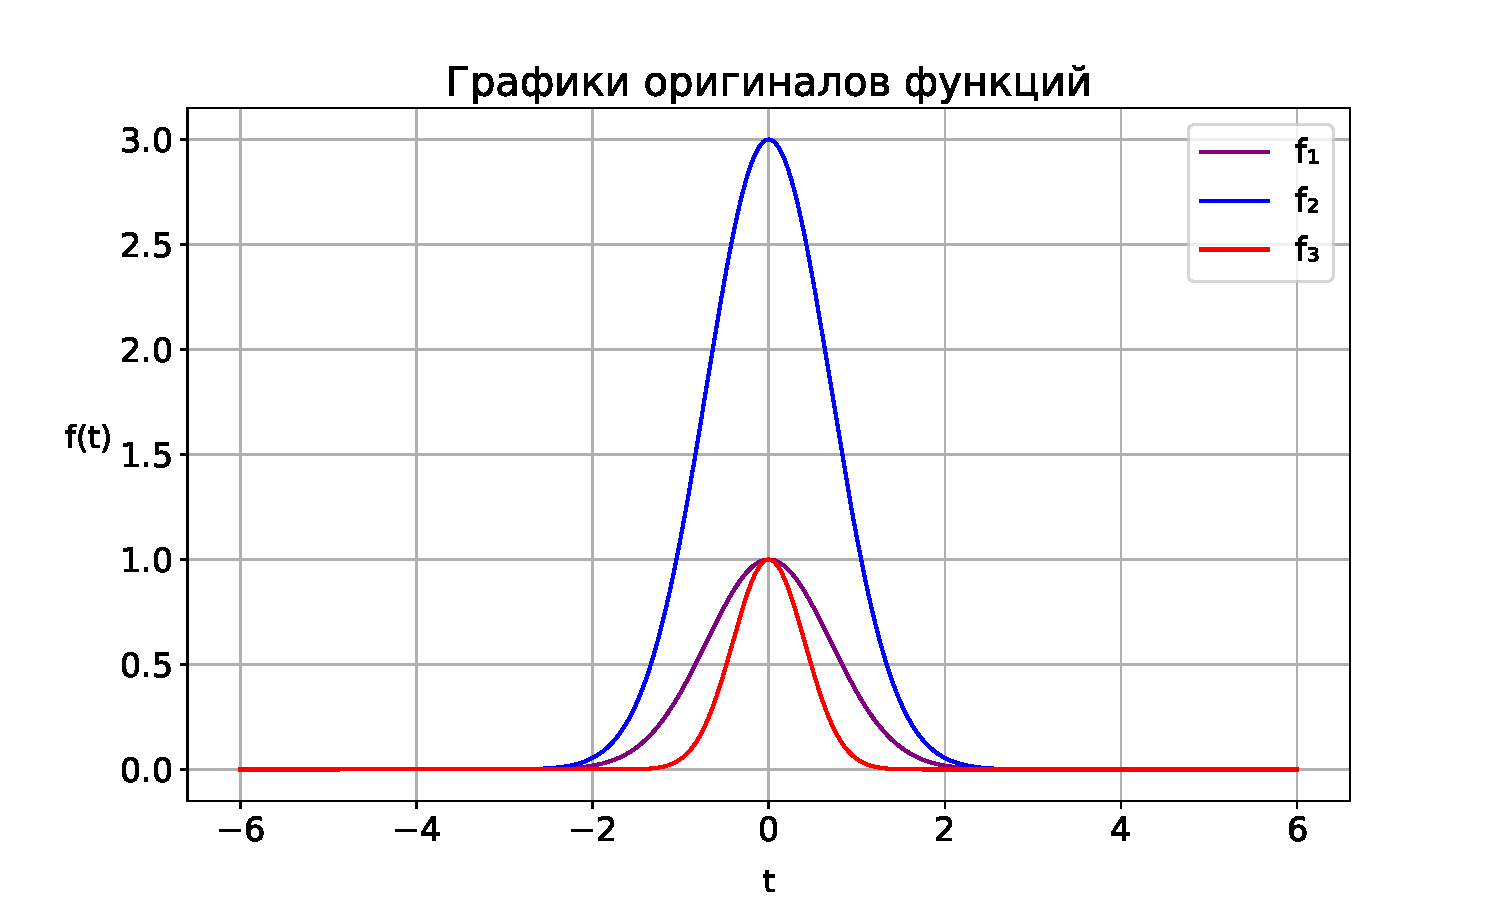
\includegraphics[width=1\linewidth]{graphs_lab2figure_1.pdf}
    \caption{Графики оригиналов функций}
    \label{fig:placeholder}
\end{figure}

\begin{figure}
    \centering
    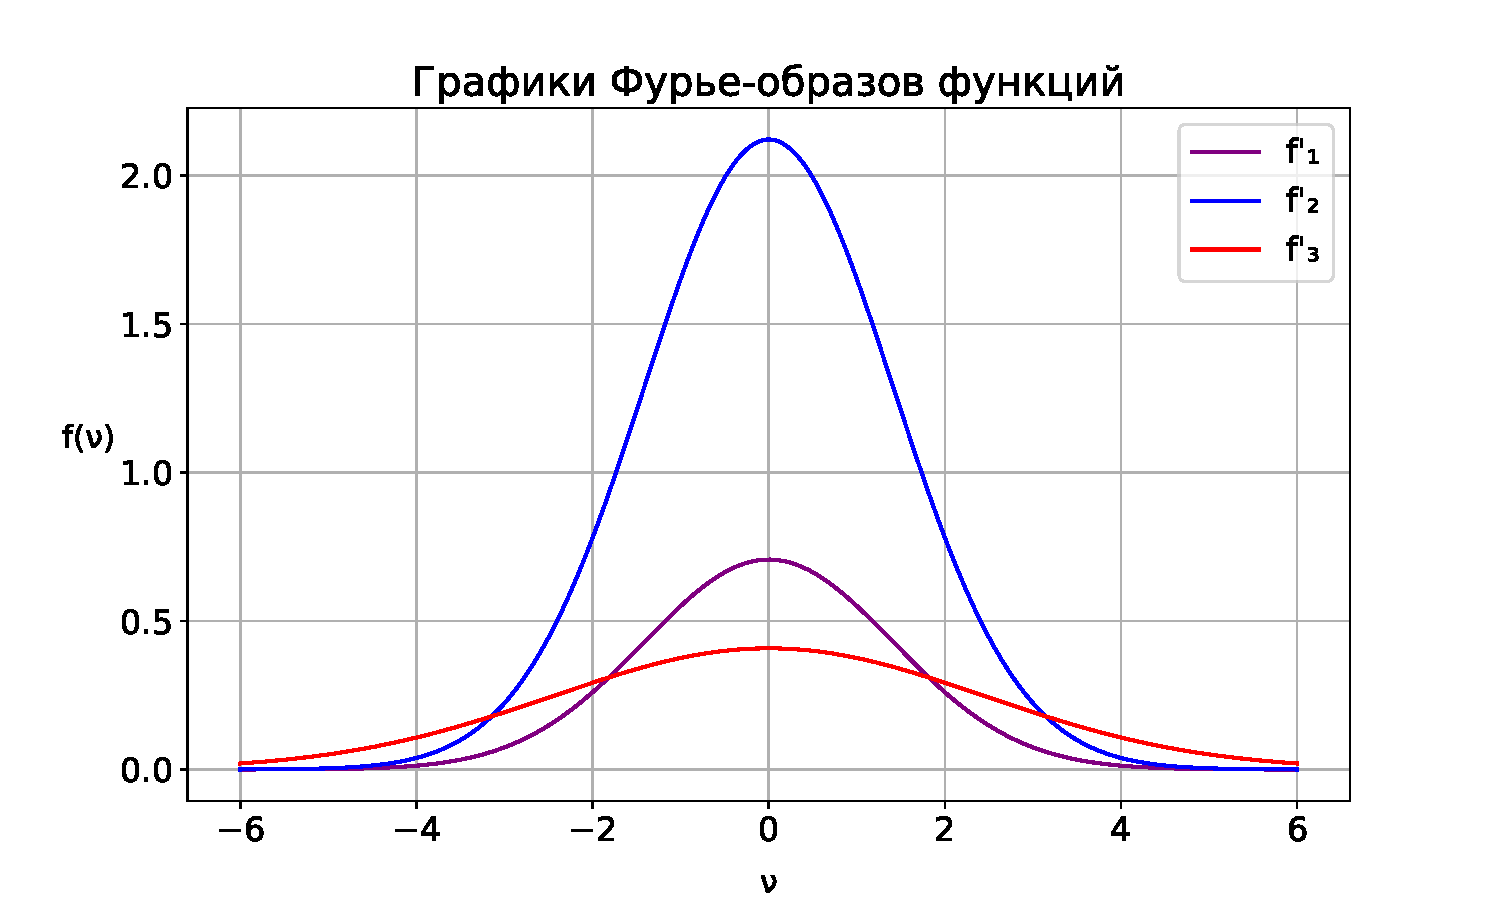
\includegraphics[width=1\linewidth]{graphs_lab2figure_2.pdf}
    \caption{Графики Фурье-образов функций}
    \label{fig:placeholder}
\end{figure}


\newpage
Параметр $a$ увеличивает амплитуду функции в $a$ раз. То есть растягивает её в $a$ раз вдоль оси $OY$\\

Параметр $b$ сжимает/растягивает функцию вдоль оси $OX$.\\

Проверим равенство Парсеваля.

\[
E_t = \int_{-\infty}^\infty a^2 e^{-2bt^2} dt = a^2 \sqrt{\frac{\pi}{2b}}.
\]

\[
E_\omega = \int_{-\infty}^\infty \frac{a^2}{2b} e^{-\frac{\omega^2}{4b}} d\omega = a^2 \sqrt{\frac{\pi}{2b}}.
\]

Равенство выполняется.

\subsection{Двустороннее затухание}
Теперь рассмотрим функцию, которая задаётся так:
\[
     f(t) = ae^{-b|t|} 
\]

Найдём её Фурье-образ:
\[
\hat{f}(\omega) = \frac{a}{\sqrt{2\pi}} \left( \int_{-\infty}^0 e^{bt} e^{-i\omega t} dt + \int_0^\infty e^{-bt} e^{-i\omega t} dt \right) = \frac{a}{\sqrt{2\pi}} \left( \frac{b + i\omega}{b^2 + \omega^2} + \frac{b - i\omega}{b^2 + \omega^2} \right) = 
\]

\[
= \frac{a}{\sqrt{2\pi}} \cdot \frac{2b}{b^2 + \omega^2}
\]

Теперь зададимся тремя наборами значений $a, b > 0$ для прямоугольной функции. Пусть $a, b = \{(1; 1),\ (1; 2),\ (2;1)\}$.\\

Построим графики для оригиналов и Фурье-образов следующих функций:

\[
{\Pi_1}(t) = e^{-|t|}  
    \ \ \ \
    \hat{f}(\omega) = \frac{1}{\sqrt{2\pi}} \cdot \frac{2}{1 + \omega^2}
\]

\[
{\Pi_2}(t) = e^{-2|t|}  
    \ \ \ \
    \hat{f}(\omega) = \frac{1}{\sqrt{2\pi}} \cdot \frac{4}{4 + \omega^2}
\]

\[
{\Pi_3}(t) = 2e^{-|t|}  
    \ \ \ \
    \hat{f}(\omega) = \frac{2}{\sqrt{2\pi}} \cdot \frac{2}{1 + \omega^2}
\]\\


\begin{figure}[H]
    \centering
    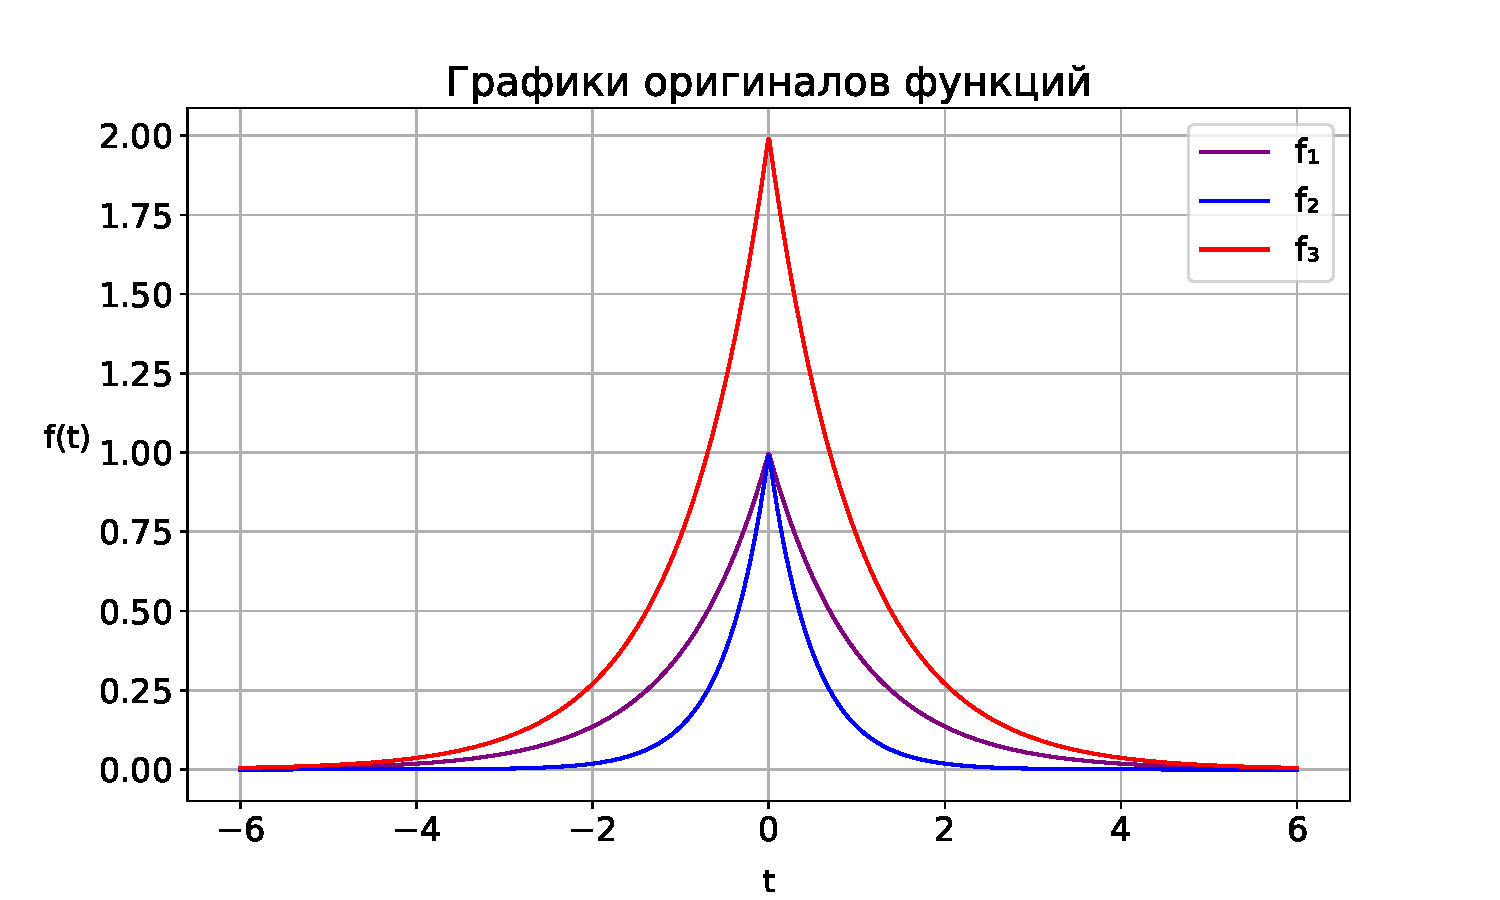
\includegraphics[width=1\linewidth]{graphs_lab2figure_3.pdf}
    \caption{Графики оригиналов функций}
    \label{fig:placeholder}
\end{figure}

\begin{figure}[H]
    \centering
    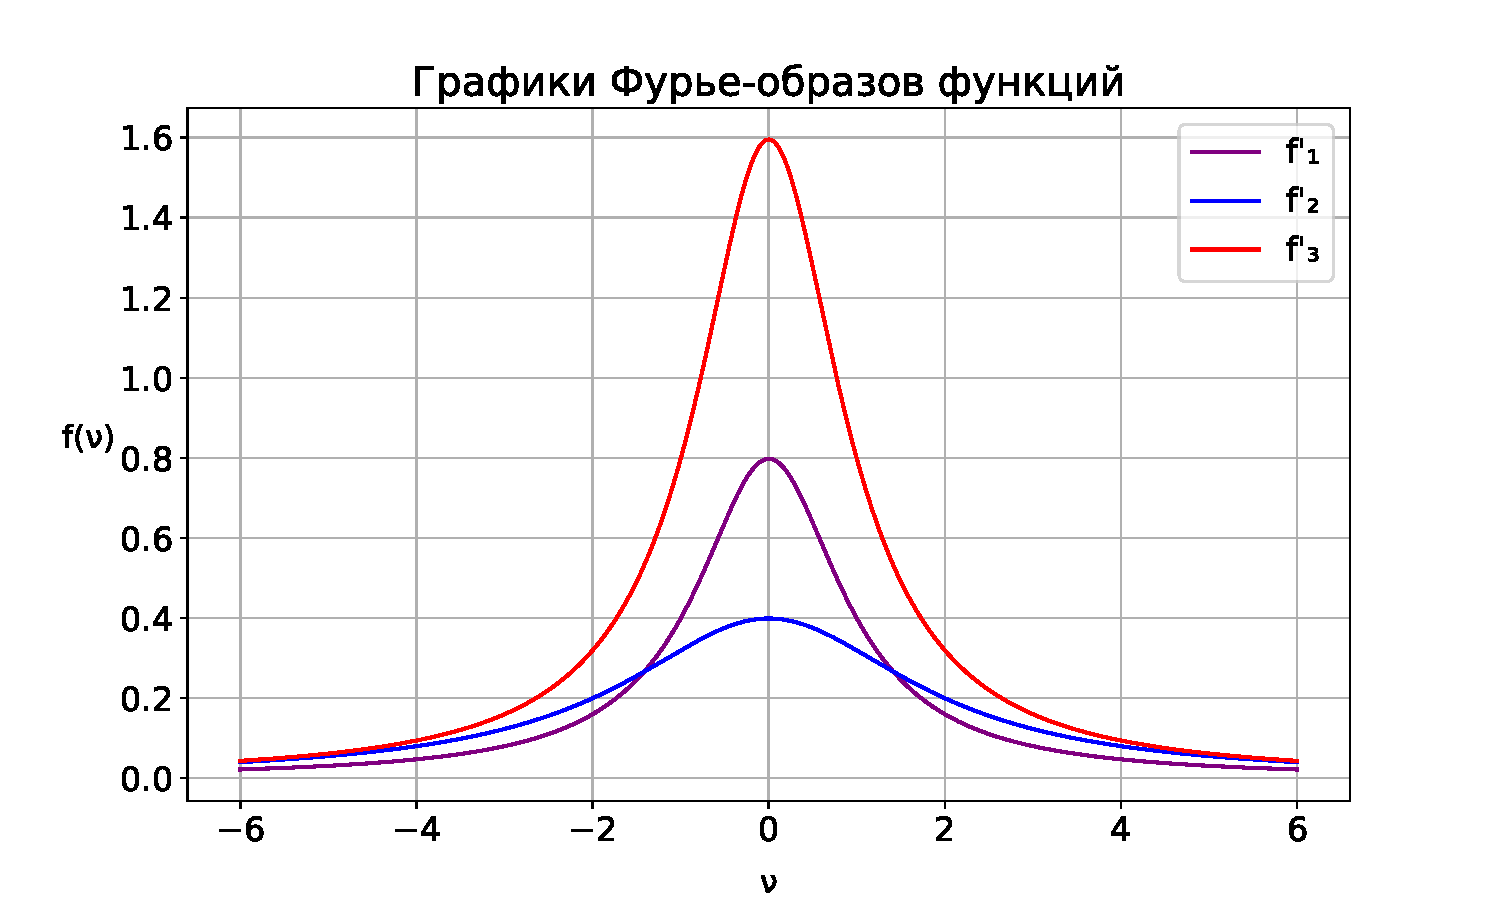
\includegraphics[width=1\linewidth]{graphs_lab2figure_4.pdf}
    \caption{Графики Фурье-образов функций}
    \label{fig:placeholder}
\end{figure}


Параметр $a$ увеличивает амплитуду функции в $a$ раз. То есть растягивает её в $a$ раз вдоль оси $OY$\\

Параметр $b$ сжимает/растягивает функцию вдоль оси $OX$.\\



\textbf{Проверка равенства Парсеваля}

\[
E_t = 2 \int_0^\infty a^2 e^{-2bt} dt = \frac{a^2}{b}.
\]

\[
E_\omega = \frac{2a^2 b^2}{\pi} \int_{-\infty}^\infty \frac{d\omega}{(b^2 + \omega^2)^2} = \frac{a^2}{b}.
\]

Равенство выполняется.

\subsection{Выводы}
В данном задании мы сначала иследовали функции и находили их Фурье-образы сначала в общем случае, а потом подставляли положительные параметры $a, b$ и исследовали, как каждый из параметров влияет на оригинал функции и на её Фурье-образ. Если параметры умножаются на функцию - они растягивают её вдоль $OY$. Если параметры в аргументе функции - они влияют на её положение относительно $OX$\\

Не всегда образы функций <<хорошо>> совпадали с их оригиналами: например, в прямоугольной функции максимальные значения функции-оригинала $\Pi_2$ (имеет синий цвет на графике) и её образа не совпадают. Похожее явление наблюдалось и в треугольной функции, и в кардинальном синусе, и во всех остальных рассматриваемых в этом задании функциях. Однако это не ошибка вычислений, ведь равенство Парсеваля везде выполнено.\\

\newpage
\section{Комплексная функция}

\subsection{Аналитические выкладки}
Рассмотрим функцию кардинальный синус из задания 1.3. Тогда функция $g(t)$ принимает следующий вид:

$$g(t) = f(t+c) = 3sinc(t+c) = \frac{3sin(t+c)}{t+c}$$

Записываем унитарное преобразование Фурье к угловой скорости $\omega$:
$$\hat g(\omega) = \frac{1}{\sqrt{2\pi}}\int_{-\infty}^{\infty}g(t)e^{-i\omega t}dt = \frac{1}{\sqrt{2\pi}}\int_{-\infty}^{\infty} 3sinc(t+c)e^{-i\omega t}dt$$

Сделаем замену:
\begin{cases}
    x = t + c \;\Leftrightarrow\; t = x - c \\
    dt = dx;\; t \rightarrow \pm \infty \Leftrightarrow x \rightarrow \pm \infty \\
    e^{-iwt} = e^{-iw(x-c)} = e^{iwc}e^{-iwx}
\end{cases}

Получаем:

$$\hat g(\omega) = \frac{e^{iwc}}{\sqrt{2\pi}}\int_{-\infty}^{\infty}3 sinc(x)e^{-i\omega x}dx$$

Зная преобразование Фурье для кардинального синуса~\eqref{equation: sinc img}, можем переписать результат:

$$\hat g(\omega) = e^{iwc} \cdot \Pi_{3, 1} (\omega),$$

где $\Pi_{a, b}(\omega) = $ 
\begin{cases}
\sqrt{\frac{\pi}{2}} \cdot \frac{a}{b} & |\omega|\le b,\\[10pt]
0, & |\omega|>b    
\end{cases},

Также можно было получить образ функции $g(t)$, если бы сразу воспользовались \textbf{свойством сдвига Фурье-оператора}: 
$${\cal F}\{f(t+c)\} = e^{iwc}\cdot{\cal F}\{f(t)\}$$

Исследование проводилось для трёх значений сдвига: $c \in \{0, 1, 2\}$.

\subsection{Результаты}

На рис.~\ref{fig:complex_originals} представлены оригиналы функции $g(t) = 3\,\mathrm{sinc}(t + c)$ для выбранных значений $c$. При $c = 0$ функция чётная. Увеличение $c$ смещает функцию влево, сохраняя её форму и амплитуду.

\begin{figure}[H] 
    
\includegraphics[width=1\textwidth]{pete-graphs/figure_3.pdf}
    \caption{Оригиналы функции $g(t) = 3\,\mathrm{sinc}(t + c)$}
    \label{fig:complex_originals}
\end{figure}

На рис.~\ref{fig:complex_fourier0},~\ref{fig:complex_fourier1},~\ref{fig:complex_fourier2} показаны компоненты Фурье-образа для всех значений $c$: вещественная часть, мнимая часть и модуль.
Вещественная~\eqref{eq:rel} и мнимая~\eqref{eq:im} части выражаются следующим образом (по формуле Эйлера):
\begin{equation}
    Re\;\hat g(\omega) = \Pi_{3, 1}\cdot cos(wc)
    \label{eq:rel}
\end{equation}
\begin{equation}
    Im\;\hat g(\omega) = \Pi_{3, 1}\cdot sin(wc)
    \label{eq:im}
\end{equation}

\begin{figure}[H] 
    \centering
    
\includegraphics[width=0.95\textwidth]{pete-graphs/figure_4.pdf}
    \caption{Фурье-образ при $c = 0$}
    \label{fig:complex_fourier0}
\end{figure}

\begin{figure}[H] 
    \centering
    
\includegraphics[width=0.95\textwidth]{pete-graphs/figure_5.pdf}
    \caption{Фурье-образ при $c = 1$}
    \label{fig:complex_fourier1}
\end{figure}

\begin{figure}[H] 
    \centering
    
\includegraphics[width=0.95\textwidth]{pete-graphs/figure_6.pdf}
    \caption{Фурье-образ при $c = 2$}
    \label{fig:complex_fourier2}
\end{figure}

\subsection{Вывод}
Модуль образа $|\hat g(\omega)|$ во всех случаях идентичен, что ещё раз подтверждает, что он определяет только частотный спектр образа, поэтому временной сдвиг не влияет на него.
Если ещё раз взглянуть на выражения~\eqref{eq:rel},~\eqref{eq:im} вещественной и мнимой частей Фурье-образа, можно заметить, что параметр $c$ содержится в $cos$ и $sin$, то есть он влияет на частоту осциляций соответствующей части. То есть сдвиг по времени изменяет фазовую структуру спектра.
\newpage
\section{Музыкальное}

\subsection{Подготовка}

Для выполнения этого задания был выбран Python. Использованы стандартные библиотеки для работы с данными (numpy, scipy) и их визуализации (matplotlib), а также librosa для работы с аудиозаписью и joblib+tempfile для оптимизации вычислений. 


Для чтения аудиозаписи как функции был выбран метод librosa.load(), по умолчанию возвращающий numpy.ndarray со значениями функции и частоту дискретизации исходной записи. Заметим, что через частоту дискретизации можно найти длину одного сэмла и получить np.linspace, содержащий массив аргументов ($t$) функции аудиозаписи:

\begin{minted}{python}
f, sr = lb.load(chord(chord_num), mono=True)
t = np.linspace(0, len(f)/sr, len(f))
\end{minted}

Переписана под Python функция для поиска Фурье-образа:

\begin{minted}{python}
def compute_Fourier_image(f, t, dV, V):
    Yarr = []
    Varr = []
    for v in np.arange(0, V, dV):
        Varr.append(v)
        Yarr.append(trapezoid(f * np.exp(-1j * 2 * np.pi * v * t), t)) 
    return (np.array(Varr), np.array(Yarr))
\end{minted}

Функция scipy.integrate.trapezoid в Python -- аналог trapz из MATLAB. Рассматриваем частоты от 16 Гц, так как при 16.35 Гц звучит первая нота в слышимом для человека диапазоне (и минимально используемая в музыкальной теории).

Отдельно автор работы отмечает оптимизацию вычислений путём кэширования результатов выполнения функции поиска Фурье-образа для ускорения выполнения программы при повторных запусках без изменения тела функции или её аргументов при вызове:

\begin{minted}{python}
from joblib import Memory
import tempfile
cache_dir = tempfile.gettempdir() + '/freq_methods/lab2/fourier_cache'
memory = Memory(cache_dir, verbose=0)

@memory.cache
def compute_Fourier_image(f, t, dV, V): ...
\end{minted}

\newpage
\subsection{Работа с аудио и анализ}

Из нашего аккорда №6 получился следующий график:

\begin{figure}[H] 
    
\includegraphics[width=1\textwidth]{pete-graphs/figure_1.pdf}
    \caption{График функции аккорда}
\end{figure}

Далее при помощи функции compute\_Fourier\_image нашли Фурье-образ. Для выявления пиков использована функция scipy.signal.find\_peaks. В качестве параметра height передали несколько перцентилей для того, чтобы выбрать наиболее подходящий порог между шумом и пиком.
Выбранные перцентили также можно увидеть на рис.~\ref{fig: task3 image}.

\begin{figure}[H] 
    
\includegraphics[width=1\textwidth]{pete-graphs/figure_2.pdf}
    \caption{График модуля образа функции аккорда}
    \label{fig: task3 image}
\end{figure}

Для выбранных перцентилей получаем слудующий вывод программы:

\begin{minted}{text}
Найдено 10 пиков, порог 0.0042. 
Содержащиеся ноты:
A3 D3 D4

Найдено 23 пиков, порог 0.0024. 
Содержащиеся ноты:
A3 A4 G#2 D4 F#4 D3

Найдено 32 пиков, порог 0.0020. 
Содержащиеся ноты:
A3 F#3 A4 G#2 D4 F#4 D3
\end{minted}

% Некоторые базовые знания музыки позволяют провести более подробный анализ результатов
Так как автор данной части работы увлекается музыкой, он решил эмпирическим путём выяснить, что из себя представляет Аккорд №6: при помощи гитары и слуха был подобран аккорд Ре-Мажор и определены составляющие ноты (Ля малой октавы, Ре малой и первой октав и Фа-Диез первой октавы, они же A3, D3, D4, F\#4), которые стали ориентиром при анализе Фурье-образа.

Идеальной точности распознавания добиться не удалось, так как при очень больших перцентилях функция теряла одну ноту аккорда, из-за чего он становился неполным, а при уменьшении порога появлялся шум в виде нот, уже не относящихся к этому аккорду.

\begin{itemize}
    \item При пороге 0.002 (перцентиль 97\%), было обнаружено 32 пика, в котором помимо нужных нам 4 нот имеются <<выбросы>> F\#3, G\#2, A4. Данные пики могли возникнуть из-за особенностей звукоизвлечения при игре гитаре. В момент удара по струнам помимо звука зажатых струн имеется звук самого удара, который может так же проявляться пиком на графике Фурье-образа, смешиваясь с негромкими оттенками аккорда.
    \item Повысив порог до 0.0024 (перцентиль 98\%), мы смогли избавиться от одной лишней ноты! Но выбросы всё ещё остались.
    \item При пороге 0.0042 (перцентиль 99\%), мы получаем набор A3, D3, D4, что соответствует power-аккорду D5, в котором отсутствует терция (F\#/Фа-Диез). Не Ре-Мажор.
\end{itemize}

\subsection{Вывод}
При выполнении анализа пиков автором была поставлена задача добиться универсальности методов, чтобы вместо Аккорда №6 можно было выбрать любой другой и написанная программа~\ref{code: task3} с максимальной точностью позволяла распознать ноты-составляющие этого аккорда. Для этого значения Фурье-образа рассматривались как выборка некоторой величины и были предприняты попытки описать её при помощи базовых выборочных характеристик (найти центр и отдалиться на него на какую-то $\Delta$, чтобы отсечь все шумы и оставить только пики), но к сожалению иделаьной точности достичь не удалось. Вероятно для высокой точности нужно использовать методы математического анализа и рассматривать, например, производные первого порядка для фильтрации пиков.

\newpage
\section{Общий вывод}
Непрерывное преобразование Фурье позволяет преобразовать функцию от времени в функцию от частоты и в некоторых случаях упростить анализ сигнала: выявить пики, и отфильтровать шумы. В данной работе были применены ненормированные и унитарные (нормированные) непрерывные преобразования Фурье, более того этот опыт был применён в практической среде (Задание 3).

\newpage
\section{Приложения}

\subsection*{Код к заданию 2}
\begin{minted}{python}
import numpy as np
import matplotlib.pyplot as plt
from scipy.integrate import trapezoid
from scipy.signal import find_peaks

import librosa as lb

from joblib import Memory
import tempfile

plt.rcParams.update({'font.size': 16})

def save_separate_figures(extension="pdf", path=""):
    """ Saves each active matplotlib figure to a separate file. """
    # Получаем номера всех созданных фигур
    fig_nums = plt.get_fignums()

    for i in fig_nums:
        plt.figure(i)
        filename = f"figure_{i}.{extension}"
        plt.savefig(path+filename)
        print(f"Сохранен файл: {filename}")

def card_sin(t, a, b, c): 
    return a * np.sinc(b*t + c)

def analytic_Fourier_card_sin(omega, a, b, c):
    Rect = lambda w, a, b: np.where(np.abs(w) <= b, np.sqrt(np.pi/2) * a/b, 0)
    return np.exp(1j*omega*c)*Rect(omega, a, b)

a, b = 3, 1
c_values = [0, 1, 2]
t = np.linspace(-10, 10, 1000)
omega = np.linspace(-5, 5, 1000)

plt.figure(figsize=(14, 6))
for c in c_values:
    g_t = card_sin(t, a, b, c)
    plt.plot(t, g_t, label=f'c = {c}', linewidth=2)
plt.title(r"Оригиналы $g(t) = \mathrm{sinc}(t + c)$")
plt.xlabel(r"$t$")
plt.ylabel(r"$g(t)$")
plt.grid(True, alpha=0.3)
plt.legend()
plt.tight_layout()


for c in c_values:
    img_g_t = analytic_Fourier_card_sin(omega, a, b, c)

    real_part = np.real(img_g_t)
    imag_part = np.imag(img_g_t)
    modulus = np.abs(img_g_t)
    
    plt.figure(figsize=(14, 10))
    
    plt.subplot(3, 1, 1)
    plt.plot(omega, real_part, 'b-', linewidth=2)
    plt.title(rf"Фурье-образ $\hat{{g}}(\omega)$ при $c = {c}$")
    plt.ylabel(r"$\mathrm{Re}(\hat{g}(\omega))$")
    plt.grid(True, alpha=0.3)
    
    plt.subplot(3, 1, 2)
    plt.plot(omega, imag_part, 'r-', linewidth=2)
    plt.ylabel(r"$\mathrm{Im}(\hat{g}(\omega))$")
    plt.grid(True, alpha=0.3)
    
    plt.subplot(3, 1, 3)
    plt.plot(omega, modulus, 'g-', linewidth=2)
    plt.ylabel(r"$|\hat{g}(\omega)|$")
    plt.xlabel(r"$\omega$, рад/с")
    plt.grid(True, alpha=0.3)
    
    plt.tight_layout()

plt.show()
save_separate_figures(path="lab2/pete-graphs/")
\end{minted}
\label{code: task2}

\subsection*{Код к заданию 3}
\begin{minted}{python}
import numpy as np
import matplotlib.pyplot as plt
from scipy.integrate import trapezoid
from scipy.signal import find_peaks

import librosa as lb

from joblib import Memory
import tempfile

plt.rcParams.update({'font.size': 16})

def save_separate_figures(extension="pdf", path=""):
    """ Saves each active matplotlib figure to a separate file. """
    # Получаем номера всех созданных фигур
    fig_nums = plt.get_fignums()

    for i in fig_nums:
        plt.figure(i)
        filename = f"figure_{i}.{extension}"
        plt.savefig(path+filename)
        print(f"Сохранен файл: {filename}")


### ЗАДАНИЕ 3
# cache_dir = tempfile.gettempdir() + 'freq_methods/lab2/fourier_cache'
cache_dir = tempfile.gettempdir() + '/freq_methods/lab2/fourier_cache'
memory = Memory(cache_dir, verbose=0)

@memory.cache
def compute_Fourier_image(f, t, dV, V):
    ImgArr = []
    vArr = []
    for v in np.arange(16, V, dV):
        vArr.append(v)
        ImgArr.append(trapezoid(f * np.exp(-1j * 2 * np.pi * v * t), t)) 
    return (np.array(vArr), np.array(ImgArr))

chord = lambda n: f'lab2/chords/Аккорд ({n}).mp3'
chord_num = 6
f, sr = lb.load(chord(chord_num), mono=True)
t = np.linspace(0, len(f)/sr, len(f))
plt.figure(figsize=(14, 6))
plt.title(r"График функции $f(t)\;-\;$" + f"Звуковая волна аккорда №{chord_num}")


plt.plot(t, f, linewidth=0.5)
plt.xlabel(r"$t$, сек")
plt.ylabel(r"$f(t)$")
plt.tight_layout()
dv = 0.1
V = 500
Varr, Yarr = compute_Fourier_image(f, t, dv, V)
ampl = np.abs(Yarr)


# sorted_ampl = np.sort(ampl)
# cumsum = np.cumsum(sorted_ampl)
# cumsum /= cumsum[-1]
# plt.figure()
# plt.grid()
# plt.plot(cumsum*100, sorted_ampl)



# log_ampl = np.log10(ampl + 1e-15)
# plt.figure()
# plt.semilogy(Varr, ampl)




plt.figure(figsize=(12, 8))
plt.title(r"График модуля образа $|\hat f(\nu)$|")
plt.grid()
notes = set()
for p in [1, 2, 3]:
    threshold = np.percentile(ampl, 100 - p)
    peaks, _ = find_peaks(ampl, height=threshold)
    print(f"\nНайдено {len(peaks)} пиков, порог {threshold:.4f}. \nСодержащиеся ноты:")
    plt.plot(Varr, [threshold]*len(Varr), label=f"Порог {threshold:.4f} при перцентиле {100-p}%", linewidth=1.5)
    for freq in sorted(Varr[peaks]):
        note = lb.hz_to_note(freq)
        notes.add(note)
        # print(f"  {freq:7.2f} Hz → {note}")
    print(*notes)

# threshold = (np.quantile(ampl, 0.75) + (np.quantile(ampl, 0.75) - np.quantile(ampl, 0.25))* 1.5)*3
# threshold = np.max(ampl)*0.15
# # threshold = np.percentile(ampl, 0.9)
# print(threshold)
# peaks, props = find_peaks(ampl, height=threshold)
# note_freq = Varr[peaks]
# # print(note_freq)
# freq_values = list(props.values())
# # print(freq_values)
# for i in range(0, len(note_freq)):
#     note = lb.hz_to_note(note_freq[i])
#     print(f"{note_freq[i]:0.2f}Hz: интенсивность {freq_values[0][i]:.3f}; note {note}")

plt.plot(Varr, ampl, label="График образа аккорда", linewidth=2.5)

plt.xlabel(r"$\nu$, Гц")
plt.ylabel(r"|$\hat f(\nu)$|")
plt.legend()
plt.tight_layout()
# plt.show()
\end{minted}
\label{code: task3}

\end{document}
